\section{Introduction}
In this section, we will discuss about the goal of the project, the different component used, the assumptions made and model chosen.

\subsection{Goal of this project}
The aim of this project was to design and implement an embedded system. To do so, we decided to create an Arduino controlled traffic light crossroad. In this system, many hypothesis regarding the crossroad properties will be made and will be explain more deeply in the next sections.

We also decided to join the Embedded Software project and the Formal verification of computer systems project.

\subsection{Crossroad assumptions}

We first had to choose a traffic crossroad to implement. We strongly took inspiration from the Fraiteur crossroad (Boulevard du triomphe and Beaulieulaan) near Delta metro station.

\begin{figure}[!ht] \label{fig:crossroad}
  \centering
    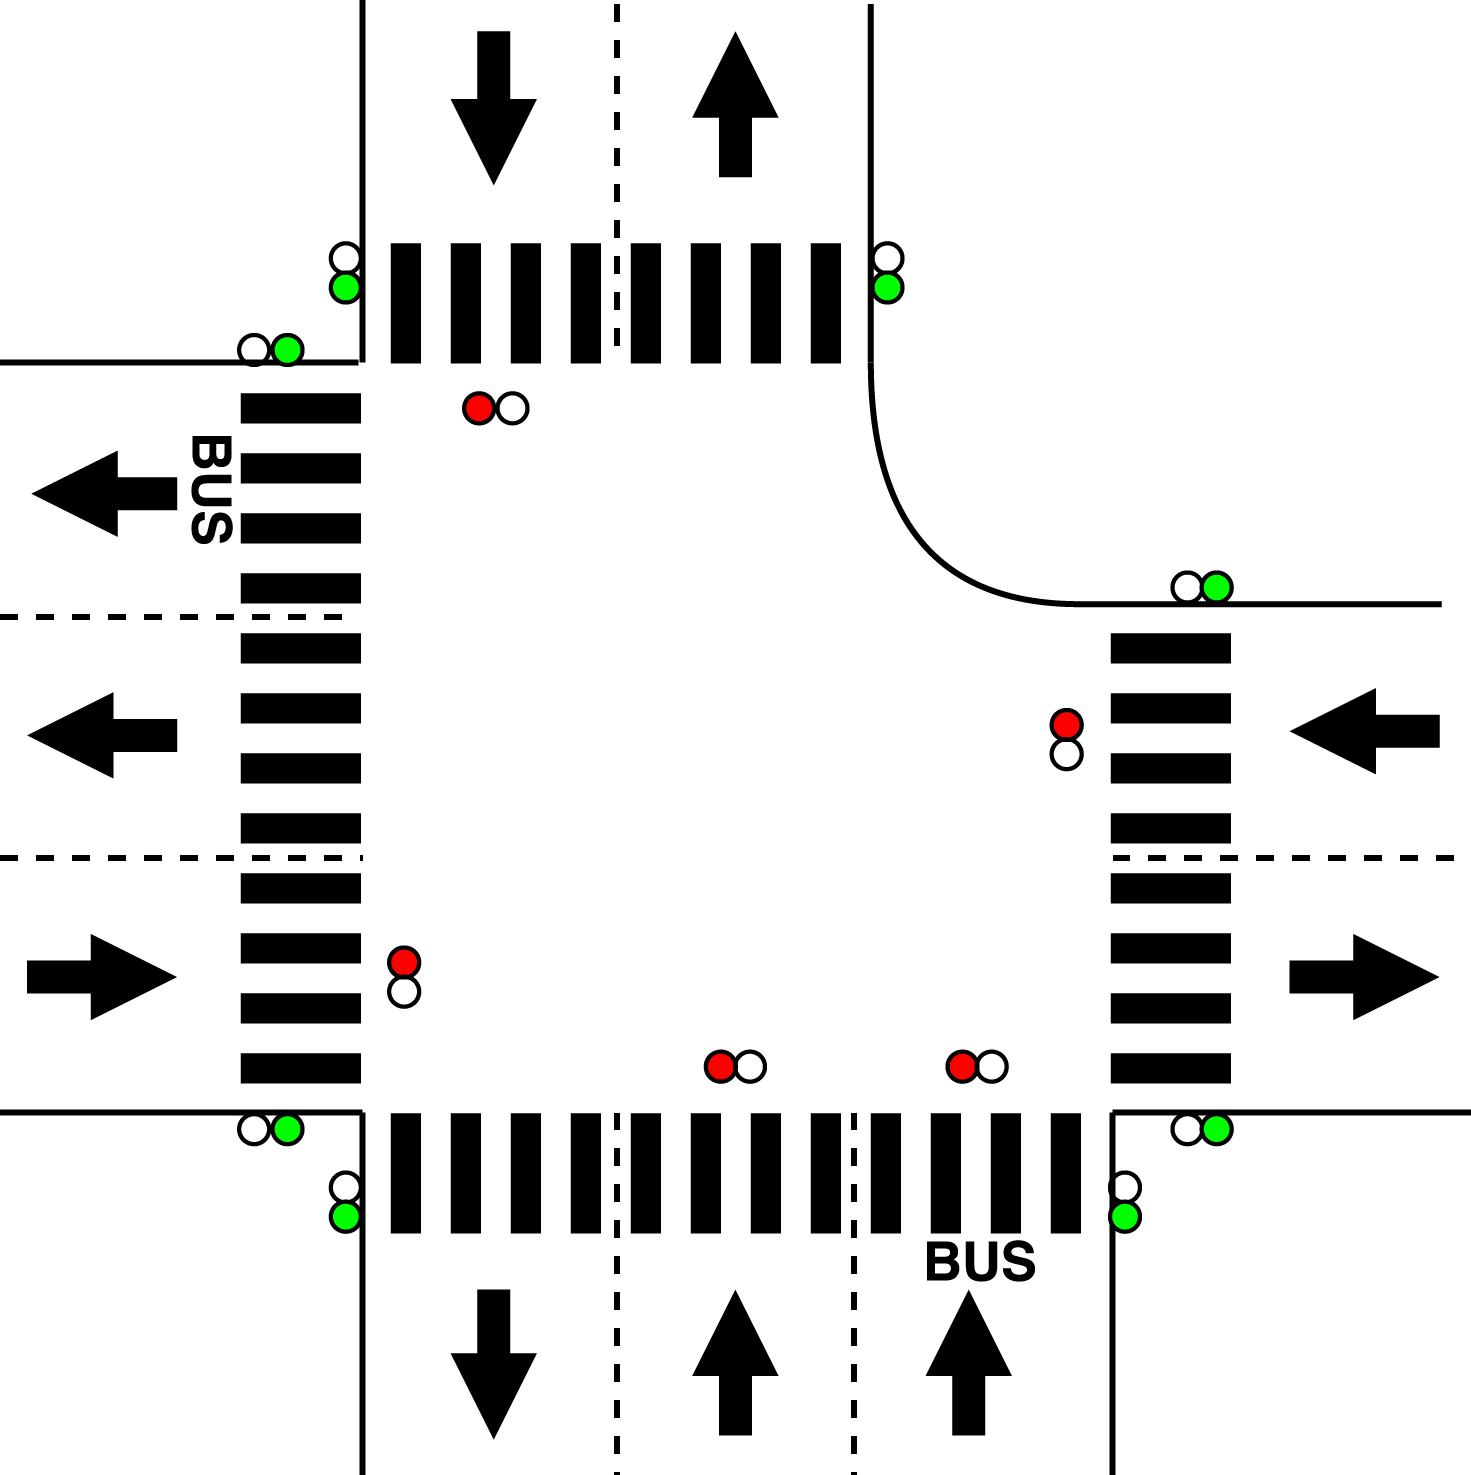
\includegraphics[width=0.7\textwidth]{picture/crossroad.png}
    \caption{The crossroad model chosen}
\end{figure}

Before defining the different actors and components in our system, some important assumptions about our model have to be taken:
\begin{itemize}
    \item The different vehicles will respect the Highway Code. This for example means that if a car is turning left and there are car on the opposite direction going straight, the car will stop to let the other pass and will turn after.
    \item At any time, a pedestrian can push a button to cross the street. There is no priority for pedestrian that would push the button many times in a row.
    \item The pedestrians will cross the street within the given time. This also means that they follow the laws and rules.
    \item All the pedestrians light are connected, that means that when pedestrian can cross, all other lights are red.
    \item As for the pedestrians, the vehicles will also cross the street within a given time.
    \item A bus can arrive at any time.
    \item If there is a bus and a pedestrian arriving at the same time, bus call take the upper hand.
\end{itemize}

\subsection{Actors}
In this section, the different actors interacting with the system will be reviewed. Those include pedestrians, buses and traffic lights.

\subsubsection{Pedestrians}
As shown on Figure \ref{fig:crossroad}, there are four different crosswalks in our model.  To make a call for the pedestrians to cross, a push button has been implemented on the controller. This means that when one pedestrian has pushed one of the button of the crossroad, the call has been made for all the pedestrians from all the sides of it. When the call is accepted by the system, the pedestrians can walk freely in the crossroad because all the lights for the cars and the buses will be red. This also means that if no pedestrians are pushing the button, meaning that no pedestrians are present, their traffic lights will always be red so the cars will always be able to drive through the crossroad.
To summarize, when the pedestrians can cross, no other vehicles can drive and have thus to wait for the red light to be green. 

\subsubsection{Buses}
The buses in our model can only go from the South path of the crossroad to the West part of it. Those buses will be created thanks to an outside event, like a pushbutton or a proximity detector. When a bus is coming, it will have a priority on every other actors. This means that when a bus has arrived in the crossroad, because it has to go through all the other lanes, the traffic lights for everyone have to be red.

\subsubsection{Traffic Lights}
In our embedded systems, traffic lights can be green or red.We purposely remove the orange light from a common belgian crossroad model because it allows us to avoid having too much cables and leds. We consider that when a traffic light is green, cars are going through the crossroad and respect the Highway Code. Cars are thus, in our model, not really an actor since they are not created, we just assume them to pass through the crossroad when their traffic lights are green. 

There are some assumptions we made about the traffic lights that are important, because we wanted fairness in our system. For example, even if the pedestrians can always push the button to have the ability to walk through the crosswalk, they have to wait that at least all other traffic lights for the cars have been green once between two green light. This means that, if no buses come and pedestrians are always pushing the button, the crosswalk with allow the cars of each side to go trough once before the pedestrians can cross again. Thanks to that, each elements in the model can't have only red light.

Another assumption is, like in common belgian crossroad, that when the South light is green, the North light is also green. On the contrary, when the East light is green, the West light is green. This means that South-North and East-West direction will have synchronized lights.

\subsubsection{Connection with Formal Verification}
We decided to combine those two projects together because they follow the same idea and we believe the two classes to be complementary and thus doing a merged project will allows us to study all side of the project, from a model to an implementation trough verification.

For the embedded project, we had to modelize an environment, and generate a controller based on that model to avoid unwanted situations through winning strategies, computed with timed games. 

For the formal verification course, a more formal approach was taken. We also had to modelize the system, but also to verify that the model was compliant to some specific properties. 

\subsection{Arduino}

To test our critical system on a real life environment, we decided to implement it with an arduino, leds and button.

We believe it to be a nice exercice because first, for most of us, it was the first time we build something using a micro-controller. Then as we witness it, micro-controller are subject to external unwanted event, like a inducted current in a cable or a button with a badly made pull-up resistor that create an event that should not have taken place. That forces us to create a strong system that can handle all of that.
